%-----------------------------------
% Plan de test simplifié
%
% ProSE
%
% Auteurs : Camille CONSTANT, Paul TRÉMOUREUX, Théo BÉNARD
%
%-----------------------------------

\documentclass[a4paper,11pt,titlepage,french]{article}
\usepackage[english,main=french]{babel}
\usepackage[T1]{fontenc}
\usepackage{lmodern}
\usepackage[utf8]{inputenc}
\usepackage{xspace, graphicx}
\usepackage{amsmath}
\usepackage{amsfonts}
\usepackage{amssymb}
\usepackage{lastpage}
\usepackage{array}
\usepackage{tabularx}
\usepackage{hyperref}
\usepackage{slashbox}
\usepackage{longtable}
\usepackage{caption}

%----------------------------------------
%       MISE EN PAGE
%----------------------------------------
\usepackage{fancyhdr}
\pagestyle{fancy}
\setlength{\hoffset}{-40pt}
\setlength{\topmargin}{-25pt}
\setlength{\headsep}{10pt}
\renewcommand{\headheight}{80pt}
\renewcommand{\headwidth}{450pt}
\setlength{\textwidth}{450pt}
\setlength{\textheight}{604pt}
\renewcommand{\footrulewidth}{0.1mm}
\fancyhf{}
        \fancyhead[LO]{\bf \includegraphics[width=80pt]{figures/eseo.png} \\ 
                \medskip 
                ProSE équipe B1 2024} 
        \fancyhead[RO]{\bf 
\includegraphics[width=90pt]{figures/logo_kereval.png} \\ 
                Ref. PlanDeTest\_B1}   

        \fancyfoot[LO]{\sl {\it Version {\versionPdT} }} 
        \cfoot{\copyright 2024 Droits réservés {\equipe}} 
        \fancyfoot[RO]{\thepage/\pageref{LastPage}}

\setcounter{tocdepth}{3}

%----------------------------------------
%       MACROS (à changer)
%----------------------------------------
\newcommand{\amodifier}{{\it À compléter et/ou modifier\\}}
\newcommand{\equipe}{CANvengers}
\newcommand{\projet}{ProSE}
\newcommand{\produit}{Passerelle Android-CAN vers banc CAN réel ou simulé}
\newcommand{\client}{KEREVAL}
\newcommand{\rqt}{Paul TRÉMOUREUX}
\newcommand{\cdp}{Théo BÉNARD}
\newcommand{\versionPdT}{2.0.0}
\newcommand{\versionProjet}{2.0.0}
\newcommand{\refSpec}{[SPEC\_B1]}
\newcommand{\refPAQL}{[PAQL\_B1\_2024]}
\newcommand{\appliC}{CANgateway}
\newcommand{\appliA}{CANdroid}

%----------------------------------------
%       DOCUMENT
%----------------------------------------
\begin{document}
%---------------------------------------
\sloppy%
% Modifie l’espacement vertical entre les lignes d’un tableau (tabular)
\renewcommand{\arraystretch}{1.5}
%---------------------------------------
\begin{center}%
{\Large {\textsc{\bf Plan de Test Système}}}
\vspace{0.4cm}\\
{\large\bf \equipe}
\vspace{0.4cm}\\
\rule[0.5ex]{0.52\textwidth}{0.1mm} \\
\vspace{0.2cm}
{\large\bf{Responsable du document : {\rqt}}}
\vspace{0.2cm}\\
{\large\bf{État du document : Validé}}
\vspace{0.2cm}\\
{\large\bf\textit{Version : {\versionPdT}}}
\end{center}
\vspace{-0.2cm}
\noindent\rule[0.5ex]{\textwidth}{0.1mm}
\newpage

% Auteurs : Camille CONSTANT, Paul TRÉMOUREUX, Théo BÉNARD

%\noindent
% Modifie l'espacement horizontal entre les colonnes
%\setlength{\tabcolsep}{5pt}
\begin{longtable}[l]{|p{2cm}|p{5.6cm}|p{2.9cm}|p{1.5cm}|p{1.7cm}|}
    \hline
        \textbf{Date} & \textbf{Actions} & \textbf{Auteur} & \textbf{Version} & \textbf{Révision}  \\
    \hline
        05/03/2019 & Création de la trame du Plan de Test. & Camille \newline CONSTANT & 0.1 & 1\\
    \hline
        22/02/2021 & Modification des critères d'acceptation, ajout des exemples de diagramme d'activité, ajout de la section Validation du document & Camille \newline CONSTANT & 0.2 & 1\\
    \hline
        03/03/2022 & Mise à jour des logiciels utilisés & Camille \newline CONSTANT & 0.2 & 2\\
    \hline
        29/03/2022 & Modification des critères d'acceptation et mention de la couverture fonctionnelle & Camille \newline CONSTANT & 0.2 & 3\\
    \hline
        06/03/2023 & Modifications pour mieux coller à la norme ISO 829-2008 & Camille \newline CONSTANT & 0.3 & 1\\
    \hline
        10/03/2023 & Mise à jour du document & Théo \newline BÉNARD & 0.4 & 0\\ 
    \hline
        15/03/2023 & Prise en main du document & Paul \newline TRÉMOUREUX & 0.4 & 1\\
    \hline
        16/03/2023 & Corrections suite au consulting test du 16/03/2023 & Paul \newline TRÉMOUREUX & 0.4 & 2\\
    \hline
        16/03/2023 & Relecture avant consulting & Paul \newline TRÉMOUREUX & 0.5 & 0\\
    \hline
        17/03/2023 & Corrections suite à l'audit consultatif du 17/03/2023 & Paul \newline TRÉMOUREUX & 0.5 & 1\\
    \hline
        21/03/2023 & Suite et fin corrections suite à l'audit consultatif du 17/03/2023 & Paul \newline TRÉMOUREUX & 0.5 & 2\\
    \hline
        22/03/2023 & Modification de l'utilisation de symbole & Paul \newline TRÉMOUREUX & 0.5 & 3\\
    \hline
        01/05/2023 & Début de correction suite aux remarques du client & Paul \newline TRÉMOUREUX & 0.5 & 4\\
    \hline
        13/05/2023 & Relecture finale de l'incrément 1 & Paul \newline TRÉMOUREUX & 0.6 & 0\\
    \hline
        15/05/2023 & Relecture globale du document & Théo \newline BÉNARD & 1.0 & 0\\
    \hline
        24/05/2023 & Modification du document pour l'incrément 2 & Paul \newline TRÉMOUREUX & 1.0 & 1\\
    \hline
        25/05/2023 & Dernières modifications du document pour l'incrément 2 & Paul \newline TRÉMOUREUX & 1.0 & 2\\
    \hline
        25/05/2023 & Relecture avant l'audit normatif & Paul \newline TRÉMOUREUX & 1.1 & 0\\
    \hline
        30/05/2023 & Début correction suite AN & Paul \newline TRÉMOUREUX & 1.1 & 1\\
    \hline
        31/05/2023 & Fin correction suite AN & Paul \newline TRÉMOUREUX & 1.1 & 2\\
    \hline
        06/06/2023 & Corrections suite relecture de Théo BÉNARD & Paul \newline TRÉMOUREUX & 1.2 & 0\\
    \hline
        12/06/2023 & Validation du document & Paul \newline TRÉMOUREUX & 2.0 & 0\\
    \hline
\end{longtable}

\captionof{table}{Table des évolutions et validations internes du document}
\newpage
%------------------------------- 
\tableofcontents
% alternative pour réduire l'espacement entre les entrées de la table des matières
% (la valeur numérique peut être adaptée au besoin) : 
%{\setlength{\baselineskip}{0.96\baselineskip}\tableofcontents\par}
\newpage
%-------------------------------
% Auteurs : Camille Constant, Paul Trémoureux

\section{Introduction}
\label{sec:intro}

\subsection{Contexte}
\label{sec:intro:contexte}

\noindent\begin{tabularx}{\linewidth}{|p{3.5cm}|X|}
\hline
{\bf Produit à tester :} & {\projet} - version {\versionProjet}\\
\hline
{\bf Type de produit :} & {\produit}.\\
\hline
{\bf Commanditaire :} & {\client}\\
\hline
{\bf Développeur :} & {\equipe}\\
\hline
{\bf Testeur :} & {\equipe}\\
\hline
\end{tabularx}

\subsection{Objet}
\label{sec:intro:objet}

Ce document décrit l'activité de test système qui sera menée par {\equipe} durant le projet {\projet} dans le but de valider le produit suivant : {\produit}. Il est rédigé sous la responsabilité du Responsable Qualité-Test (RQT), sous la direction du Chef de Projet (CdP), conformément au Plan d'Assurance Qualité Logicielle (PAQL) élaboré sous la responsabilité du RQT (cf. section~\ref{sec:eqTest}, Équipe de test).

\subsection{Portée} 
\label{sec:intro:portee}

Sont concernés par ce document :
\begin{itemize}
    \item les testeurs : afin que ceux-ci connaissent le périmètre des tests (ce qu'ils vont tester), l'environnement de test (comment les tests seront mis en {\oe}uvre) et le processus de test (comment s'y prendre et rendre compte des résultats lors de l'exécution des tests) ;
    \item les développeurs : à titre informatif, afin que ceux-ci sachent comment va être validée leur production ; à titre indicatif afin qu'ils sachent, par la description de la gestion des anomalies, comment ils s'interfaceront avec l'équipe de test ;
    \item le client : ce plan de test fait l'objet d'une contractualisation avec le client pour déterminer le périmètre des tests menés pour valider le produit livré et les niveaux d'acceptation de cette validation ;
    \item les auditeurs : ce plan de test, ainsi que son implication, feront l'objet d'audits par la société Formato.
\end{itemize}

\subsection{Copyright}
\label{sec:intro:copyright}
Cf. {\refPAQL} (section 1.3. Copyright).

\subsection{Présentation du système} 
\label{sec:intro:scope}

Le système développé est un ensemble de 2 programmes : une application Android nommé {\appliA} déployé sur un smartphone Android et un programme C nommé {\appliC} déployé sur une Raspberry Pi.
L'application {\appliA} sera relié au programme {\appliC} par un réseau TCP/IP. La Raspberry Pi sera connectée à un réseau CAN pour dialoguer avec Tableau de Bord (soit banc de test physique soit simulateur sur un PC).
Ce projet permettra d'envoyer des trames depuis l'application {\appliA} vers Tableau de Bord afin de piloter ce dernier à distance.

\subsection{Références}
\label{sec:intro:ref}

\subsubsection{Documents de référence internes}
\noindent\begin{tabularx}{\linewidth}{|p{3cm}|X|p{1.4cm}|X|}
\hline
\textbf{Ref.} & \textbf{Nom et auteur} & \textbf{Version} & \textbf{Source}\\
\hline
{\refSpec} & Dossier de spécifications - \newline {\equipe} & 2.0.0 & se2024-b1.doc/specification/livrables\\
\hline
%Si client impliqué dans le PAQL
{\refPAQL} & Plan d'Assurance Qualité Logiciel - {\rqt} & 1.0.0 & pdf sur le dépôt\\
\hline
\end{tabularx}

\subsubsection{Documents de référence externes}
\noindent\begin{tabularx}{\linewidth}{|p{2.8cm}|X|}
\hline
\textbf{Ref.} & \textbf{Nom} \\
\hline
[ISO-829-2008] & Documentation de test logiciel\\
\hline
[ISO/IEC/IEEE 29119-1:2022] & Ingénierie du logiciel et des systèmes - Essais du logiciel - Partie 1: Concepts généraux\\
\hline
\end{tabularx}

\subsection{Glossaire et abréviations}
\label{sec:intro:termes}

Ce sont les termes et abréviations nécessaires à la compréhension de l'activité de test (les termes techniques propres au projet seront indiqués dans le dossier de spécification).

\subsubsection{Abréviations}

\noindent\begin{longtable}[c]{|p{.20\textwidth}|p{.80\textwidth}|}
\hline
CdP & Chef de Projet\\
\hline
IHM & Interface Homme-Machine\\
\hline
PAQL & Plan Assurance Qualité Logicielle\\
\hline
RQT & Responsable Qualité et Test\\
\hline
\end{longtable}

\subsubsection{Glossaire}

\noindent\begin{longtable}[c]{|p{.20\textwidth}|p{.80\textwidth}|}
\hline
{\bf Campagne de test} & Activité qui consiste à dérouler un ensemble de jeux de test. Un dossier de test est produit à l'issue d'une campagne.\\
\hline
{\bf Cas de test} & Déclinaison d'un test précisant les valeurs utilisées pour les variables du test ainsi que les résultats attendus.\\
\hline
{\bf Dossier de test} & Ensemble documentaire qui contient la description des scénarios et des cas de tests, ainsi que l'exécution des jeux de test. Le dossier de test est le reflet d'une campagne de test. \\
\hline
{\bf Jeux de test} & Ensemble des scénarios et cas de tests permettant de tester un produit logiciel. L'enchaînement des cas et scénarios de tests est relatif à une stratégie de test précisée dans le plan de test.\\
\hline
{\bf Plan de test} & Document décrivant le déroulement d'un jeu de test : stratégie de test, critères d'arrêt, planification.\\
\hline
{\bf Scénarios de test} & Ensemble de cas de tests cohérents permettant de traiter un objectif fonctionnel.\\
\hline
{\bf Test d'intégration} & Vérification effectuée pour montrer des défauts dans les interfaces et interactions de composants ou systèmes intégrés.\\
\hline
{\bf Test de non régression} & Vérification qu'une nouvelle version du produit fonctionne sans dégradation (technique, fonctionnelle, performance) par rapport à la version précédente.\\
\hline
{\bf Test de validation} & Vérification que le produit est cohérent et complet par rapport aux spécifications fonctionnelles.\\
\hline
{\bf Test fonctionnel} & Test (vu de l'utilisateur) du bon fonctionnement d'un produit logiciel, d'une fonctionnalité ou d'une fonction de base. Vérification par rapport aux spécifications.\\
\hline
{\bf Test système} & Vérification que le système dans son ensemble est cohérent et complet par rapport aux spécifications fonctionnelles et techniques.\\
\hline
{\bf Test unitaire} & Vérification que les composants logiciels individuels sont cohérents et complets par rapport aux spécifications.\\
\hline
\end{longtable}

Voir également le \href{https://www.cftl.fr/wp-content/uploads/2018/10/Glossaire-des-tests-logiciels-v3_2F-ISTQB-CFTL-1.pdf}{[Glossaire CFTL/ISTQB des termes utilisés en tests de logiciels]}.\\

\subsection{Conformité}
\label{sec:intro:conf}

Ce plan de test est conforme aux normes~:

\begin{itemize}
    \item IEEE Std. 1012-1986
    \item ISO Std. 829-2008
    \item IEEE Std. 1008-1987
    \item ISO/IEC/IEEE 29119-1:2022
\end{itemize}
\newpage

% Auteurs : Camille Constant, Paul Trémoureux

\section{Périmètre de test}
\label{sec:perimetre}
Cette section a pour objet l'élaboration d'un tableau des fonctionnalités et/ou composants/traitements/données du système mentionnant pour chacun l'effort de test à mener.
Cet effort est fonction de la pondération des exigences, risques et criticité retenus.

\subsection{Caractéristiques du projet}
\label{sec:peri:caract} 

KEREVAL, une entreprise spécialisée dans les tests de systèmes embarqués dans les véhicules, souhaite développer un démonstrateur CAN \og simulator in the loop \fg pour permettre à ses équipes de monter en compétences sur le réseau CAN.\\

L'objectif est également de fournir une visualisation concrète de l'architecture du véhicule, du réseau CAN et du démonstrateur CAN pour les personnes qui débutent dans le métier, tels que les nouveaux salariés lors de leur arrivés chez KEREVAL, ou des étudiants lors de forums.\\

Pour répondre à ce besoin, KEREVAL souhaite pouvoir utiliser un simulateur de tableau de bord sur Linux (type ICSim) et/ou un banc de test physique connecté(s) à une carte électronique (type Raspberry Pi) pour permettre la connection au réseau CAN, à la fois réels (sur le banc de test fourni par KEREVAL) et simulés (par le simulateur de tableau de bord).\\

De plus, KEREVAL souhaite contrôler le système à distance via une application Android nommée {\appliA} déployée sur un smartphone. Ce dernier sera connecté au système (via la Raspberry Pi) par un réseau TCP/IP. Sur l'application, il sera possible d'envoyer et d'enregistrer des trames mais également d'observer toutes les trames diffusées sur le bus CAN. Il sera possible d'enregistrer les trames diffusées sur le bus dans un fichier présent sur la Raspberry Pi.\\

En outre, l'entreprise souhaite être en mesure d'injecter des fautes via les trames pour s'assurer du bon fonctionnement du démonstrateur.\\

%Le produit {\produit} permet à {\client} d'étudier la faisabilité de...\\

Le projet {\projet} se décompose en 2 lots/incréments~:
\begin{itemize}
    \item Lot 1~:
    \begin{itemize}
        \item Communication TCP/IP (entre le programme {\appliC} et l'application {\appliA}) :
        \begin{itemize}
            \item Envoi de trame depuis l'application {\appliA}
            \item Reception de trame sur l'application {\appliA}
        \end{itemize}
        \item Communication CAN (entre le programme {\appliC} et Tableau de Bord) :
        \begin{itemize}
            \item Sniffer fonctionnel sur le programme {\appliC}
            \item Communication avec Simulateur ICSim
        \end{itemize}
        \item Gestion du SàE :
        \begin{itemize}
            \item Démarrer le SàE
        \end{itemize}
    \end{itemize}
    \item Lot 2~:
    \begin{itemize}
        \item Communication CAN (entre le programme {\appliC} et Tableau de Bord) :
        \begin{itemize}
            \item Communication avec Banc de Test
        \end{itemize}
        \item Gestion des objets sur l'application {\appliA} :
        \begin{itemize}
            \item Création d'objets sur l'application {\appliA}
            \item Création de trames dans un objet sur l'application {\appliA}
            \item Mode d'envoi
            \item Suppression d'objets sur l'application {\appliA}
            \item Suppression de trames dans un objet sur l'application {\appliA}
        \end{itemize}
        \item Gestion du sniffer sur l'application {\appliA} :
        \begin{itemize}
            \item Pause du sniffer sur l'application {\appliA}
            \item Nettoyage du sniffer sur l'application {\appliA}
            \item Retour en haut du sniffer sur l'application {\appliA}
        \end{itemize}
        \item Gestion de la communication sur l'application {\appliA} :
        \begin{itemize}
            \item Reconnexion
        \end{itemize}
        \item Gestion du SàE :
        \begin{itemize}
            \item Stopper le SàE
        \end{itemize}
    \end{itemize}
\end{itemize}
\medskip

{\client} souhaite connaître la qualité globale de \og {\produit} \fg après chaque lot afin d'éventuellement redéfinir chacun des lots. \\
Ce plan de test concerne le niveau de test système. Pour information, des tests d'intégration (lots 1 et 2) et des tests unitaires (lot 2) auront été réalisés par {\equipe}.

\subsection{Éléments à tester}
\label{sec:peri:elements} 

Cette partie s'appuie sur la section \og 2.3 Fonctions principales développées \fg du document de spécifications {\refSpec}. 
\medskip

%{\it Faire classement par catégories (logiciels développés, supports d'exécution (logiciels et matériels), supports de communication (logiciel (ex : pile TCP/IP) et matériel)).}
Les éléments à tester se décomposent en plusieurs catégories~:
\begin{itemize}
    \item Logiciels développés :
    \begin{itemize}
        \item L'application {\appliA}
        \item Le programme {\appliC}
    \end{itemize}
    \item Support de communication :
    \begin{itemize}
        \item Protocole de communication
    \end{itemize}
\end{itemize}

\subsubsection{Éléments concernés par les tests}
\label{sec:peri:comp:test}
          
Cette section désigne ce qui est testé (composant, logiciel, sous-système).
Seront concernés par l'activité de test les composants logiciels développés durant le projet {\projet}: le programme {\appliC} et l'application {\appliA}, ainsi que la couche application de la communication entre le programme {\appliC} et l'application {\appliA} (+ drivers si développés). 

\subsubsection{Éléments non concernés par les tests}
\label{sec:peri:comp:nontest}

Cette section désigne ce qui ne va pas être testé (composant, logiciel, sous-système).\\
Ne seront pas concernés par les tests les supports d'exécution logiciels (Linux, Android, librairies, etc.) et matériels (E\_Smartphone, E\_Raspberry, E\_BancTest et E\_ICSim) ainsi que les supports de communication matériels (E\_PC, E\_PEAK, E\_Shield) et logiciels (pile TCP/IP). 

\subsection{Spécifications fonctionnelles ou techniques à tester}
\label{sec:peri:spec}

Cette section s'appuie sur la section 2.3 du document de spécifications {\refSpec}.
Cette section s'appuie également sur la matrice Fonctionnalités-CUs [MatriceFonctionnalitesCUTests.pdf].

\subsubsection{Fonctionnalités à tester}
\label{sec:peri:fct:test}

Les fonctionnalités suivantes sont à tester (avec les paramètres et jeux de données prédéfinis):
\noindent\begin{longtable}[c]{|p{.40\textwidth}|p{.20\textwidth}|p{.40\textwidth}|}
\hline
\bf Fonctionnalité & \bf \centering Priorité & \bf Commentaire\\
[-1ex] & (P0 : priorité max) & \\
\hline
\endhead
Envoi de trames depuis l'application {\appliA} & \centering P0 & L'utilisateur doit pouvoir demander l'envoi de trames depuis l'application {\appliA}. L'application {\appliA} doit être capable d'envoyer des trames vers le programme {\appliC}.\\
\hline
Réception de trames sur l'application {\appliA} & \centering P0 & L'application {\appliA} doit être capable de recevoir des trames depuis le programme {\appliC}.\\
\hline
Sniffer fonctionnel sur le programme {\appliC} & \centering P0 & Le programme {\appliC} doit être capable de lire sur le réseau CAN.\\
\hline
Communication avec Banc de Test & \centering P5 & Le programme {\appliC} doit être capable de communiquer avec Banc de Test via le réseau CAN.\\
\hline
Communication avec Simulateur ICSim & \centering P1 & Le programme {\appliC} doit être capable de communiquer avec Simulateur ICSim via le réseau CAN.\\
\hline
Création d'objets sur l'application {\appliA} & \centering P2 & L'utilisateur doit pouvoir créer un objet sur l'application {\appliA}. L'application {\appliA} doit être capable d'afficher cet objet.\\
\hline
Création de trames dans un objet sur l'application {\appliA} & \centering P2 & L'utilisateur doit pouvoir créer une trame dans un objet sur l'application {\appliA}. L'application {\appliA} doit être capable d'afficher cette trame dans l'objet.\\
\hline
Mode d'envoi & \centering P3 & L'utilisateur doit pouvoir choisir le mode d'envoi de la trame créée sur l'application {\appliA}. L'application {\appliA} doit être capable d'envoyer les trames selon leurs modes d'envoi.\\
\hline
Suppression d'objets sur l'application {\appliA} & \centering P4 & L'utilisateur doit pouvoir supprimer un objet sur l'application {\appliA}. L'application {\appliA} doit être capable d'enlever cet objet de l'affichage.\\
\hline
Suppression de trames dans un objet sur l'application {\appliA} & \centering P4 & L'utilisateur doit pouvoir supprimer une trame dans un objet sur l'application {\appliA}. L'application {\appliA} doit être capable d'enlever cette trame de l'affichage de l'objet.\\
\hline
Pause du sniffer sur l'application {\appliA} & \centering P2 & L'utilisateur doit pouvoir demander la pause du sniffer sur l'application {\appliA}. L'application {\appliA} doit pouvoir mettre en pause la reception des trames dans le sniffer.\\
\hline
Nettoyage du sniffer sur l'application {\appliA} & \centering P3 & L'utilisateur doit pouvoir demander le nettoyage du sniffer sur l'application {\appliA}. L'application {\appliA} doit pouvoir effacer les trames afficher dans la partie sniffer de l'application {\appliA}.\\
\hline
Enregistrement du sniffer dans un fichier de log & \centering P2 & L'utilisateur doit pouvoir demander sur l'application {\appliA} l'enregistrement des trames reçues dans un fichier. L'application {\appliA} doit pouvoir enregistrer les trames reçues dans un fichier.\\
\hline
Retour en haut du sniffer sur l'application {\appliA} & \centering P4 & L'utilisateur doit pouvoir demander sur l'application {\appliA} de revenir en haut de l'affichage des trames du sniffer. L'application {\appliA} doit pouvoir revenir en haut de l'affichage des trames du sniffer.\\
\hline
Reconnexion & \centering P2 & L'utilisateur doit pouvoir demander sur la reconnexion de l'application {\appliA} avec le programme {\appliC}. L'application {\appliA} doit pouvoir se reconnecter avec le programme {\appliC}.\\
\hline
Démarrer le SàE & \centering P0 & L'utilisateur doit pouvoir démarrer le SàE.\\
\hline
Stopper le SàE & \centering P2 & L'utilisateur doit pouvoir stopper le SàE.\\
\hline
Redémarrer le SàE & \centering P2 & L'utilisateur doit pouvoir redémarrer le SàE. Le SàE doit permettre une persistance des données.\\
\hline
\end{longtable}

\subsubsection{Caractéristiques techniques à tester}
\label{sec:peri:tech:test}

Cette section s'appuie sur la section \og 2.4 Contraintes \fg du document de spécifications {\refSpec}.\\
%<exigences non fonctionnelles> du document de spécifications {\refSpec}. \\
Les caractéristiques techniques suivantes sont à tester :
\noindent\begin{longtable}[c]{|p{.40\textwidth}|p{.20\textwidth}|p{.40\textwidth}|}
\hline
\bf Caractéristique & \bf \centering Priorité & \bf Commentaire\\
[-1ex] & (P0 : priorité max) & \\
\hline
\endhead
%En commantaires les caractéristiques à ajouter à l'incrément 2
Fiabilité & \centering P1 & Le système doit être robuste aux arrêts/redémarrages/coupures électriques.\\
\hline
Ergonomie & \centering P1 & Le sous-système application Android doit être ergonomique. Les règles d'ergonomie ont été échangées avec KEREVAL.\\
\hline
Facilité d'utilisation & \centering P0 & Le sous-système application Android doit être intuitif, i.e. prise en main et utilisation sans documentation.\\
\hline
Facilité d'utilisation & \centering P1 & Le sous-système application Android doit permettre à l'utilisateur de savoir dans quel état est le système complet (état de marche, en erreur, en mode dégradé).\\
\hline
Lisibilité message & \centering P0 & Les messages d'erreur doivent être compréhensibles, doivent permettre de diagnostiquer le système et le remettre dans un état opérationnel.\\
\hline
Performance en sortie & \centering P1 & Les actionneurs doivent répondre en moins de 1 seconde suite à une sollicitation via le sous-système application Android (temps de prise en compte d'une commande).\\
\hline
Performance en entrée & \centering P1 & Une information capteur est affichée en moins de 1 seconde sur le sous-système application Android (temps de remontée d'une information capteur).\\
\hline
Maintenabilité & \centering P1 & L'architecture du système doit être modulaire et permettre de remplacer/d'ajouter des capteurs/actionneurs commandables via l'application Android.\\
\hline
\end{longtable}

\subsection{Spécifications fonctionnelles ou techniques non testées}
\label{sec:peri:nontest}

L'ergonomie ainsi que la conformité de l'emplacement des éléments de l'IHM aux spécifications ne sera pas testée. L'IHM ne sera validée qu'au travers des tests fonctionnels. 
Le fonctionnement du tableau de bord type banc de test, de ses actionneurs et de ses voyants ne sera pas testé.
L'ensemble des éléments listés dans la partie \og \ref{sec:peri:comp:nontest} Éléments non concernés par les tests \fg de ce document ne seront pas testés.\\

Les caractéristiques techniques suivantes ne seront pas testées :
\noindent\begin{longtable}[c]{|p{.50\textwidth}|p{.50\textwidth}|}
    \hline
    \bf Caractéristique & \bf Commentaire\\
    \hline
    \endhead
    Sécurité & Le système doit implémenter les bonnes pratiques de sécurité imposées par les développements sécurisés.\\
    \hline
    Portabilité système & Le sous-système application Android peut être portable sur les différentes versions Android, à partir de version 9.\\
    \hline
    Portabilité matériel & Le sous-système application Android peut être portable sur les smartphones supportant une version 9 ou supérieure.\\
    \hline
    Eco-conception & Le système ne doit pas consommer plus que la valeur vue avec le client.\\
    \hline
\end{longtable}

\subsection{Criticité}
\label{sec:peri:criticite}

Les éléments suivants revêtent une importance critique :
\begin{itemize}
    \item La communication entre le programme {\appliC} et l'application {\appliA} ;
    \item La communication entre le programme {\appliC} et la partie tableau de bord.
\end{itemize}

\subsection{Risques}
\label{sec:peri:risques}

\noindent Id : identifiant du risque\\
Description : description du risque\\
Effet : effet du risque\\
P : probabilité (3 - très probable, 2 - probable, 1 - peu probable)\\
I : impact (3 - impact fort, 2 - impact moyen, 1 - impact faible)\\
EI (élément impacté) : coût/qualité/délai\\
Action : description de l'action pour maîtriser le risque

\subsubsection{Risques projet}
\label{sec:peri:risques:projet}

\noindent\begin{longtable}[c]{|p{1.4cm}|p{3cm}|p{3cm}|p{0.4cm}|p{0.4cm}|p{1.2cm}|p{3.5cm}|}
\hline
\bf Id & \bf Intitulé & \bf Effet & \bf \centering P & \bf \centering I & \bf \centering EI & \bf Action\\
\hline
\endhead
RPRJ1 & Pas de test unitaire & Instabilité de l'application lors des tests système & \centering 2 & \centering 2 & \centering C/Q/D & Faire une phase de smoke tests sur l'application avant de réaliser les tests système.\\
\hline
RPRJ2 & Pas de test d'intégration & Instabilité de l'application lors des tests système & \centering 1 & \centering 2 & \centering C/Q/D & Faire une phase de smoke tests sur l'application avant de réaliser les tests système.\\
\hline
RPRJ3 & Pas de test unitaire ou de test d'intégration & Instabilité de l'application lors de tests d'acceptation & \centering 1 & \centering 2 & \centering C/Q/D & Réaliser des tests système sur toutes les fonctionnalités système.\\
\hline
RPRJ4 & Problème de disponibilité des intervenants & Dérive dans le planning des tests & \centering 1 & \centering 1 & \centering D & Planifier au plus tôt les actions des différents intervenants.\\
\hline
RPRJ5 & Spécifications du produit \og {\produit} \fg non à jour & Déviations entre les spécifications et le système d'où une difficulté pour concevoir des tests pertinents & \centering 1 & \centering 2 & \centering Q & Analyse des spécifications pour identifier des écarts. Poser toutes les questions nécessaires à une bonne compréhension des spécifications.\\
\hline
RPRJ6 & Non respect des règles inscrites dans le PAQL & Conflits de noms/dépots sur le RDP. Baisse de la qualité de la production. & \centering 2 & \centering 1 & \centering Q & Activité de contrôle régulier des productions de l'équipe.\\
\hline
\end{longtable}

\subsubsection{Risques produit}
\label{sec:peri:risques:produit}

\noindent\begin{longtable}[c]{|p{1.4cm}|p{3cm}|p{3cm}|p{0.4cm}|p{0.4cm}|p{1.2cm}|p{3.5cm}|}
\hline
\bf Id & \bf Intitulé & \bf Effet & \bf \centering P & \bf \centering I & \bf \centering EI & \bf Action\\
\hline
\endhead
RPRD1 & Mauvaise implémentation de la communication & Système non fonctionnel & \centering 1 & \centering 3 & \centering C/Q/D & Tester la communication en priorité par des tests d'intégrations (voir unitaires) avant de faire les tests système.\\
\hline
RPRD2 & Dysfonctionnement du matériel (Tableaux de Bord (type Banc de Test)) & Système non fonctionnel & \centering 2 & \centering 2 & \centering C/Q/D & Formation à l'utilisation du matériel. Aide de {\client}.\\
\hline
RPRD3 & Dysfonctionnement du matériel (Smartphone, Raspberry PI, Tableaux de Bord (type Simulateur), Connecteurs CAN) & Système non fonctionnel & \centering 1 & \centering 3 & \centering C/Q/D & Formation à l'utilisation du matériel, redondance et bouchonnage.\\
\hline
\end{longtable}

\subsection{Effort de test}
\label{sec:peri:effort}

L'effort de test sera priorisé de la façon suivante :
\begin{itemize}
    \item Phase de \og Smoke test \fg pour vérifier la stabilité de l'application avant de réaliser la campagne de tests fonctionnels système ;
    \item Campagne de tests fonctionnels système par priorité ;
    \item Campagne de tests non fonctionnels système par priorité.
\end{itemize}
\newpage

% Auteurs : Camille Constant, Paul Trémoureux

\section{Processus et Stratégie de test}
\label{sec:process}

\subsection{Objectifs (actions de test)}
\label{sec:process:objectifs}

\noindent Exigence : exigence concernée\\
Risque : risque concerné (cf. section \ref{sec:peri:risques})\\
Niveau : niveau de test (S : Système, I : Intégration, U : Unitaire)\\
Technique : technique de test (AP : Analyse Partitionnelle ou Classes d'équivalence, AL : Analyse aux limites, CU : Cas d'Utilisation, PC : Protocole de Communication)\\

\noindent\begin{longtable}[c]{|p{0.5cm}|p{2.8cm}|p{1.7cm}|p{1.2cm}|p{1.2cm}|p{1.8cm}|p{3.6cm}|}
\hline
\bf \centering N\textdegree & \bf Énoncé de l'objectif & \bf Exigence & \bf Risque & \bf Niveau & \bf Technique & \bf Conditions de mesure/niveau d'atteinte prévu.\\
\hline
\endhead
\centering 1 & Tester la communication & Fonct. P0 & RPRD1 & I, S & AP, PC, CU & Fonctionnalités P0/100\% des fonctionnalités testées en utilisant les classes d'équivalence, le protocole de communication et les cas d'utilisation.\\
\hline
\centering 2 & Smoke test & Toutes & RPRJ1, RPRJ2, RPRJ4 & S & Test par expérience & Nombre d'anomalies bloquantes/pas d'anomalie bloquante.\\
\hline
\centering 3 & Tester 100\% des fonctionnalités P0 & Fonct. P0 & RPRJ3, RPRD1 & S & AP, CU & Fonctionnalités P0/100\% des fonctionnalités testées en utilisant les classes d'équivalence et les cas d'utilisation.\\
\hline
\centering 4 & Tester 100\% des fonctionnalités non P0 & Fonct. non P0 & RPRJ3, RPRD1 & S & AP, CU & Nombre de cas d'utilisation/tous les cas d'utilisation testés.\\
\hline
\centering 5 & Contrôle qualité des productions. & Toutes & RPRJ6 & U & Relecture, PAQL & Respect des règles du PAQL.\\
\hline
\end{longtable}

\subsection{Organisation}
\label{sec:process:orga}

\subsubsection{Découpage en phase de tests/campagnes}
\label{sec:process:orga:decoupage}

Deux campagnes de tests système sont prévues dans le projet pour chaque lot/incrément :
\begin{itemize}
    \item Campagne de tests système comprenant les tests fonctionnels et non fonctionnels pour atteindre les différents objectifs de tests ci-dessus ;
    \item Campagne de retest (vérification de la correction des anomalies détectées) et de régression.
\end{itemize}

\subsubsection{Gestion des rapports d'anomalie}
\label{sec:process:orga:anomalies}

Les anomalies sont gérées dans l'ENTP sous forme de tâche.
Dès l'observation d'une défaillance dans le produit, un rapport d'anomalie est rédigé dans l'ENTP.

\subsection{Critères d'acceptation des tests}
\label{sec:process:accept}

Pour le passage en test de validation système, la phase de smoke test ne doit pas détecter d'anomalie bloquante.\\
Pour la mise en production, aucune anomalie bloquante ni majeure n'est acceptée.

\noindent\begin{longtable}[c]{|p{.25\textwidth}|p{.75\textwidth}|}
\hline
{\bf Anomalie bloquante} & La fonctionnalité n'est pas utilisable.\\
\hline
{\bf Anomalie majeure} & La fonctionnalité ne répond pas à ses exigences mais une solution de contournement existe pour utiliser la fonctionnalité, ou la fonctionnalité est utilisable en l'état (par exemple, anomalie dans une règle de calcul).\\
\hline
{\bf Anomalie mineure} & La fonctionnalité est utilisable mais pas de façon optimale (par exemple, problème d'ergonomie ou de charte graphique).\\
\hline
\end{longtable}

\subsection{Critères d'arrêt}
\label{sec:process:arret}

Les tests d'une fonctionnalité s'arrêteront si une anomalie bloquante est découverte ne permettant pas de poursuivre les tests de cette fonctionnalité.

\subsection{Activités de test}
\label{sec:process:activites}  
  
L'activité de test sera faite par {\equipe} tout au long du cycle de développement, via notamment :
\begin{itemize}
    \item Des tests de validation sur le comportement nominal et aux limites du système ;
    \item Des tests d'intégration sur le comportement nominal du programme {\appliC} ;
    %Ligne à ajouter au second incrément, ne pas oublier les modifications de ponctuation.
    \item Des tests unitaires nominaux sur certaines classes de l'application {\appliA} et sur certains modules du programme {\appliC}.
\end{itemize}

\subsubsection{Planification}

La planification des tests système est réalisée par {\equipe}.

\subsubsection{Conception}

La conception des tests système est réalisée par {\equipe}.
La conception des jeux de données de test est réalisée par {\equipe}.

\subsubsection{Exécution}

L'exécution des tests système est réalisée par {\equipe}.
L'exécution des tests d'acceptation est réalisée par {\client}.

\subsubsection{Bilan}

{\equipe} rédige un bilan de test en fin de campagne de test système.

\subsection{Documents de test et livrables}
\label{sec:process:livrables}

\noindent\begin{longtable}[c]{|l|c|}
\hline
{\bf Documentation} & {\bf Livrable à transmettre} \\
\hline
Plan de test & X \\
\hline
Dossier de test & X \\
\hline
Rapport de test & X \\
\hline
Matrice de conformité exigences et tests & X \\
\hline
Rapport d’anomalies & X \\
\hline
{\bf Données} & \\
\hline
Documents d'analyses partitionnelles et aux limites & \\
\hline
Jeux de données de tests & X\\
\hline
{\bf Automatisation des tests} & \\
\hline
Code de test & \\
\hline
\end{longtable}
\newpage

% Auteurs : Camille Constant, Paul Trémoureux 

\section{Environnement de test}
\label{sec:env}

\subsection{Environnement matériel et logiciel de test}
\label{sec:env:env}

Liste des matériels et logiciels nécessaires à l'exécution des tests :
\begin{itemize}
    \item E\_PC : Linux Ubuntu (64-bit) ;
    \item E\_Smartphone : Samsung Galaxy A20e sous système Android 9 ;
    \item E\_Raspberry : pi 3B+ ;
    \item E\_Passerelle : RS485 ;
    \item E\_ICSim : version du 12/06/2020 ;
    \item E\_PEAK : PEAK PCAN.USB IPEH-002021 175459 ;
    \item E\_Banc\_De\_Test : KEREVAL Banc de Test.
\end{itemize}

\subsection{Outils de test}
\label{sec:env:outils}

Les tests seront au maximum automatisés grâce aux outils suivants :
\begin{itemize}
    \item Tests unitaires : Framework de test Android (basé sur JUnit), bouchonnage Mockito, CMocka ;
    \item Tests d'intégration : JMeter ;
    \item Tests de validation : automatisation avec Robot Framework, sinon tests manuels ;
    \item Dossier de test : Squash TM avec intégration de la gestion d'anomalies via Redmine.
\end{itemize}

\newpage

% Auteur : Camille Constant

\section{Rôles et responsabilités}
\label{sec:resp}

{\equipe} :
\begin{itemize}
    \item Gestionnaire de tests :
    \begin{itemize}
        \item Rédaction du plan de tests ;
        \item Rédaction du bilan de tests ;
        \item Suivi de la réalisation des tests système ;
        \item Reporting auprès de {\client}.
    \end{itemize}
    \item Analyste de tests :
    \begin{itemize}
        \item Conception des tests ;
        \item Conception des jeux de données ;
        \item Exécution des tests ;
        \item Gestion des rapports d'anomalies (création et clôture).
    \end{itemize}
\end{itemize}

{\client} :
\begin{itemize}
    \item Validation des documents produits.
    \item Réalisation de tests d'acceptation.
\end{itemize}

{\equipe} ne peut être tenu responsable des répercussions d'une défaillance d'une fonctionnalité non validée. 

\newpage

% Auteurs : Camille Constant, Paul Trémoureux 

\section{Équipe de test}
\label{sec:eqTest}

Le CdP est responsable des moyens mis à disposition pour mener à bien l'activité de test et de l'attribution des tâches.
\medskip

Le RQT est responsable de l'organisation, du déroulement de l'activité de test et de la rédaction du cahier de test.
\medskip

Les testeurs sont responsables des résultats de test reportés dans le cahier de test et du développement et implémentation des codes de test.

Les rôles au sein de {\equipe} se divisent de la façon suivante :
\noindent\begin{longtable}[c]{|p{8cm}|p{1.5cm}|p{1.5cm}|p{1.5cm}|}
\hline
    & {\bf CdP} & {\bf RQT} & {\bf Testeur} \\
\hline
Théo BÉNARD & X &   & X \\
\hline
Elisa DECLERCK &   &   & X \\
\hline
Camille LENNE &   &   & X \\
\hline
Gabriel MARQUETTE &   &   & X \\
\hline
Thomes ROCHER &   &   & X \\
\hline
Paul TRÉMOUREUX &   & X & X \\
\hline
\end{longtable}
\newpage

% Auteur : Camille Constant

\section{Planning prévisionnel}
\label{sec:planning}

\begin{figure}[ht] 
    \centering
    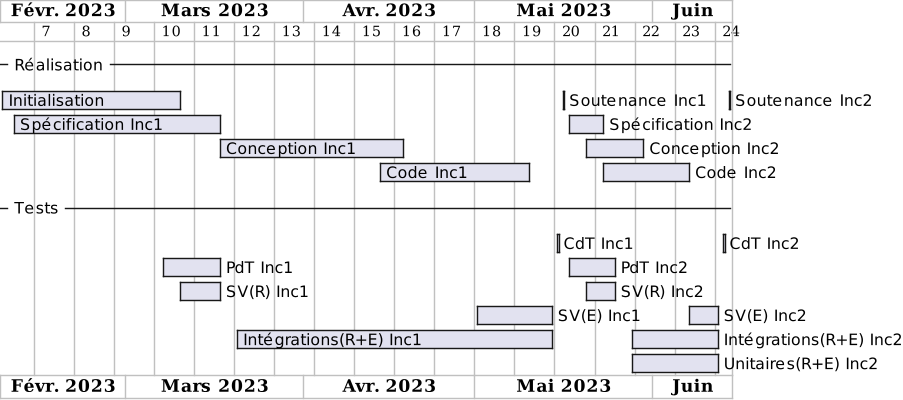
\includegraphics[width=14cm]{schemas/gantt.png}
    \caption{Diagramme de Gantt du projet {\projet}}
\end{figure}

\newpage

% Auteur : Camille Constant

\section{Validation du document}
\label{sec:validation}

\bigskip


\noindent\begin{tabularx}{\linewidth}{XX}
Document fait à & , le\\[2ex]
Pour la société \client & Pour la société \equipe \\
Mention {\guillemetleft} Lu et approuvé {\guillemetright} : & Mention {\guillemetleft} Lu et approuvé {\guillemetright} : \\[5ex]
Signature(s) : & Signature(s) : \\
\end{tabularx}
\newpage

\end{document}
%--- END